\chapter{Classification}

\section{Hardware resources}
- server for storing the training data as the results 
- 3 computers accesseed via ssh. One is more powerfull ... specs table than the other two .. specs table. These 3 computers have direct acces to the data server and load the training data from there. While the data server is optimized for storing data the other 3 computers used focus on computing power for fast training of modells. 

\section{Training setup}
- one script for training the 1D cnn and one for the 2d cnn. Only difference is in the structure of the cnns and that before training the 2d cnn the loaded statistical feaures must first be used to create the synthetic images.
- Both scripts load the same statistical features, already divided into 20 splits. As there are statistical features for 20 real and 20000 simlauted no obstacles games as well as the same amount for glare effects games, this results in each split containing data from 19 real and 19000 simualted games for each of the two classes, resulting in 38 real and 38000 simulated games available for the training. From the left out 2 real and 2000 simulated games, only the data from the real games is used for testing. This is done becauuse it is not desirable that the models adapt to the simualted data as in reality they will be only used in real games. 



- it can be chosen in a list which ratios between simualted and real games schould be traiuned. It was chosen to use 0, .. 10, 20

- it can be chosen how many steps in the game should be used. The less the faster is the decision is made and assistance can be applied, but the longer wated the better the results (likely). So modells for different amounts of steps are trained. Steps: 10, 20, 30, 40 (or in turns divide by 2). 

- vielleicht erwähnen: es ist nicht soinderlich sinvvoll nur schritte in der mitte zu nehemen, weil erstens die ersten schritte bei weniger genutzen simulationen die besten sind und andererseits das ziel der hci interaction ist so schnell wie möglich herauszufinden ob ein hinderniss stattfand. Wenn man die ersten 5 oder 10 züge ignoriert dauert dies länger.

- The structure and hyper parameters of the modells for all 1d cnns are identical. Same goes for all 2d modells. The only differnece is the input shape of the modells since it depends on teh number of steps used in the training. Identical structure for modells of the same type are used so that different training results for different amount of steps can be reliably compared. It should be noted the structure and hyper paramters are not the same between the 1d and 2d cnns. This is only important for models of the same type. 



- The scripts create and use a specific directory structure conceptualized in figure ref.

... figure 

resutls -> 2d... -> sdxordner,(sdx images) -> split1 -> run1resutls 

\begin{tikzpicture}
[sibling distance=3cm,-,thick]
\footnotesize
\node {classification results}
child {node {hi}
	[sibling distance=2cm]
	child {node {hi2.1}
		child {node {deciduous}}
		child {node {evergreen}}
	}
	child {node {...}}
	child {node {hi2.20}}
}
child {node {...}
}
child {node {...}
}
;
\end{tikzpicture}

structure erklären

- in everey iteration: multithreading 20 cores. one for each split and the resuls for each split in every iteratrion . This also means all modells are traing using the cpu. Since all used computers especially the one from table ref have many fast cores, multithreading gives fast training results and enables parallel training of multiple modells.  \todo{ich glaube das geht nicht mit gpu aber nochmal checken}.   

\section{Models}
For determining whether probands were blinded, one dimensional and two dimensional convolutional neural networks were utilized. One dimensional convolutional neural networks have become popular for time series classifications \todo{ref}. Two dimensional coovolutinal neural networks are mostly used for image processing. However, a possibility is to create synthetic images from the data and use these images in a two dimensional convolutional network. The widths of the data and the feature maps in the visualizations are calculafed for the case that all 20 rounds are used. If a diferenet nuber of rounds is used the widths are differentbut can be determined likewise \todo{klarstellen}. The cnn models are intentionally created not very complex for two reasons: Firstly, a lot of training needs to be done with differnet configurations regarding the steps includes and the ratios of simulkated to real data. As the time this work is created in is limited, training all the modells for a sufficient analysis would take too long. Especially the training of the 2d cnns requires a lot of time. Secondly, to assure that the structures are complex enough, more complex modells were exemplary trained and they showed either similar or worse performance.

\subsection{1D CNN}
The structure of the 1D CNN used is shown in figure \ref{fig:1dCnnStructure}.
\begin{figure}[H]
	\centering
	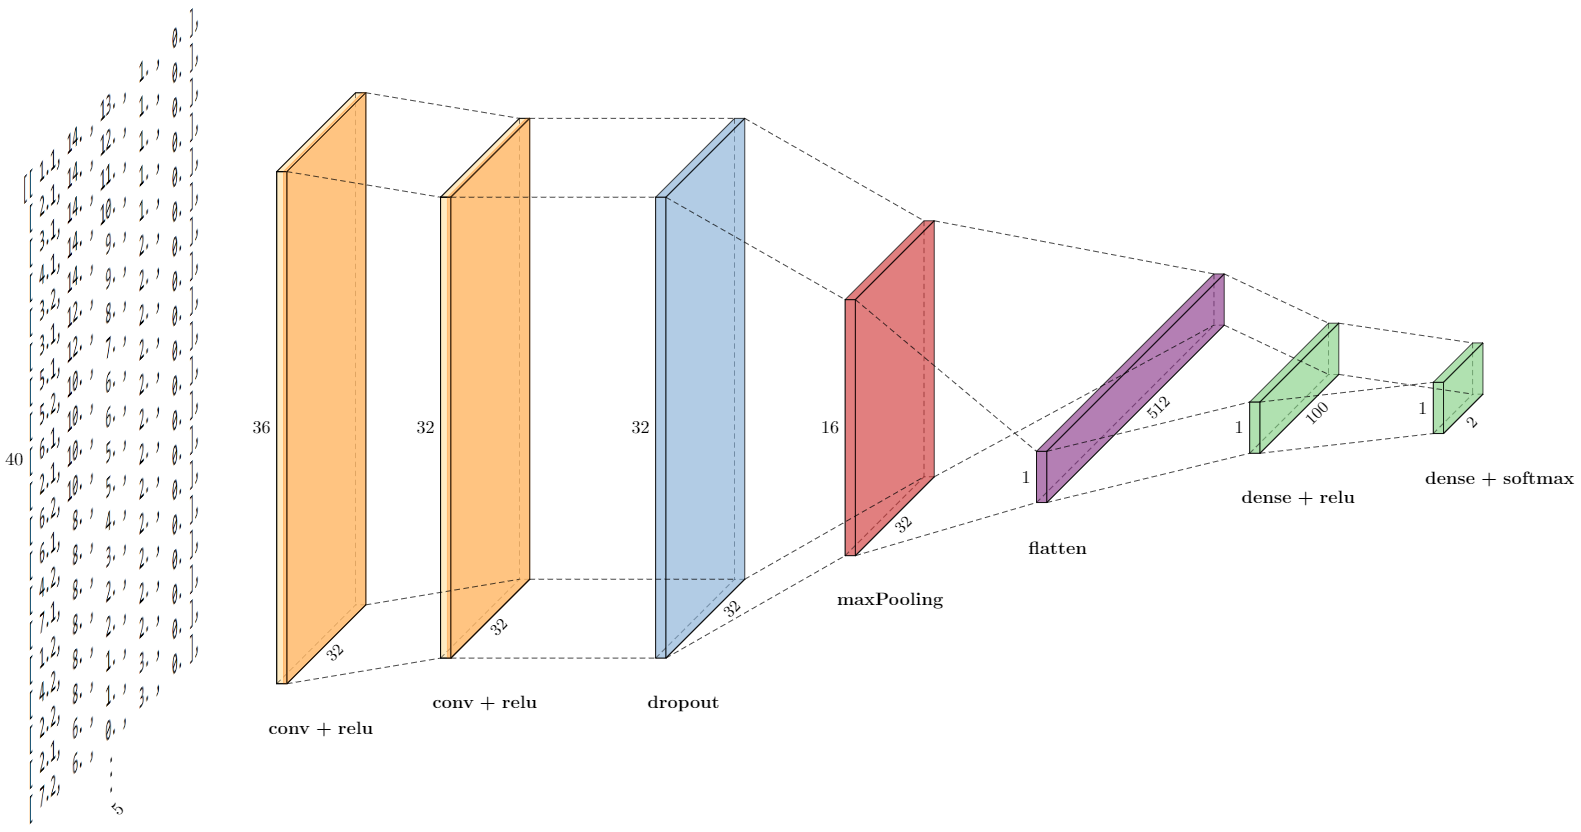
\includegraphics[width=15cm]{images/1dCnnStructure.png}
	\caption[Bild kurz]{Add caption}
	\label{fig:1dCnnStructure}
\end{figure}
\todo{anpassen an 1d cnn diagramm, weil es vorher falsch war}
The input data consist of the 5 statical features explained in .. \todo{ref} for each of the 40 steps (20 rounds), resulting in the input dimensions 40 $\cdot$ 4. Initially the data is passed to the first convolutional layer of the network. The first layer has 32 filters and the kernel has a size of 5, meaning that every step from the kernel includes all data from 5 steps in the game. This convolution results in 32 festure maps each with dimensions of 36 $\cdot$ 5. These feature maps are passed to the second convolutional layer with the same number of filters and the same kernel size as the first layer. This again results in 32 feature maps and a decresed dimensionality of 32 $\cdot$ 5. Afterwards a dropout layer with a rate of 0.5 randomly sets input units to 0 and by that helps to prevent overfitting. Then a one dimensional max pooling layer with a pool size of 2 reduces the dimensinalty to 16 $\cdot$ 5.  And finally the network is completed with a flatten layer and two dense layers \todo{vielleicht genauer erklären was dense macht, aber eigentlich ja oben auch schon, nur einen groben satz hier}. Both convolutional layers, and the first dense layer use a rectified linear unit as activation function. The last dense layer uses softmax normalization to bring the data down two two values for the two classes. The elemets of the output vector are between 0 and 1 and sum up to 1 and specify the result of the classification.  

total trainable parameters: 57.486

\subsection{2D CNN}
The structure of the 1D CNN used is shown in figure \ref{fig:2dCnnStructure}.
\begin{figure}[H]
	\centering
	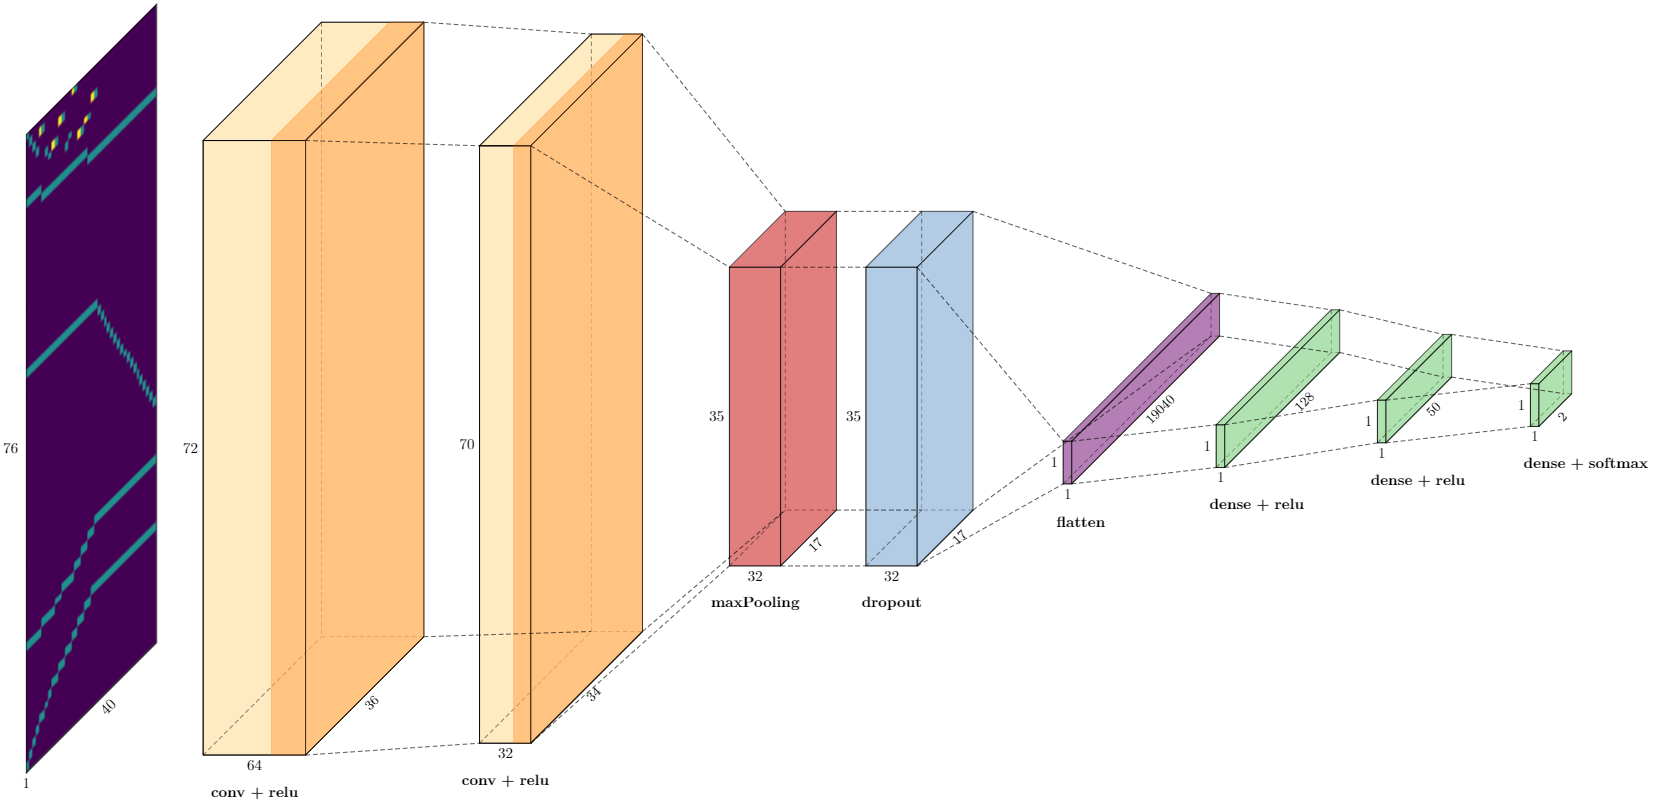
\includegraphics[width=15cm]{images/2dCnnStructure_new.png}
	\caption[Bild kurz]{Add caption}
	\label{fig:2dCnnStructure}
\end{figure}
The input data consist of the synthetic images generated in .. \todo{ref} using the 5 statistical features, resulting in the input dimensions 75 $\cdot$ 40. Initially the data is passed to the first convolutional layer of the network. The first layer has 64 filters and the kernel has a size of 5 $\cdot$ 5, meaning that each step from the kernel includes a 5 $\cdot$ 5 are of the synthetic image. This convolution results in 64 festure maps each with dimensions of 71 $\cdot$ 36. These feature maps are passed to the second convolutional layer with 32 filters and a kernel size of 3 $\cdot$ 3. This results in 32 feature maps and a decresed dimensionality of 69 $\cdot$ 34. Then a two dimensional max pooling layer with a pool size of 2 $\cdot$ 2 reduces the dimensinalty to 35 $\cdot$ 17. It is important to note that this does not happen by default. Due to the fact that 69 is odd, by default the last row would be ignored during a max pooling with dimensions 2 $\cdot$ 2 dimensions, meaning the dimensions would be 34 $\cdot$ 17 instead. As this is undesirable due to the potentially lost information in the last row, zero padding was used to create an additional row with zeros. This additional row results in the pooling not having to ignore the last row \todo{weil sich dimension auf 76 ändert stattdessen schreieb: da die height und width gerade sind und das pooling 2 mal 2 ist, wird beim pooling keine reihe oder spalte ausgelassen, es wird also kein zero padding benötigt}. Afterwards a dropout layer with a rate of 0.2 randomly sets input units to 0 and by that helps to prevent overfitting. And finally the network is completed with a flatten layer and three dense layers \todo{vielleicht genauer erklären was dense macht, aber eigentlich ja oben auch schon, nur einen groben satz hier}. Both convolutional layers, and the first two dense layers use a rectified linear unit as activation function. The last dense layer uses softmax normalization to bring the data down two two values for the two classes. The elements of the output vector are between 0 and 1 and sum up to 1 and specify the result of the classification.

total trainable parameters: 2.463.928

\begin{comment}

\subsubsection{Visualizing intermediate activations}
\todo{vielleichtz diese section rausnehemen. ich denke es ist unnötig, weil es nicht dazu beiträgt was meine arbeit zeigen soll}

An interesting thing about 2d cnns is that it is possible to vizualize the reprenestations learned by the network. This helps to understand the meaning of individual filters. Intermediate activations canm be vizualized by displaying the feauture maps that are the outpu of various convolution and pooling layers in the network, given an image is passed to the input layer. \todo{ref} To extract these feature maps, the model is first trained for one split and then run in prediction mode. Vizualizing each feature map produced by filters gives a view into how an input is decomposed into the different filters learned by the cnn. The decision was made not to focus too much on vizualizing all feature maps but instead to only vizualize one feature map created by each layer. As each feature map can learn different features, the following visualizations are only small fractions of what the cnn learns. Thgerefore they should only serve as exemplary illustration of what the different layers of the cnn output.

\todo{bisschen beschreiebn was was ist von den bildern und was man sieht}

\begin{minipage}{0.5\textwidth}
	\begin{figure}[H]
		\centering
		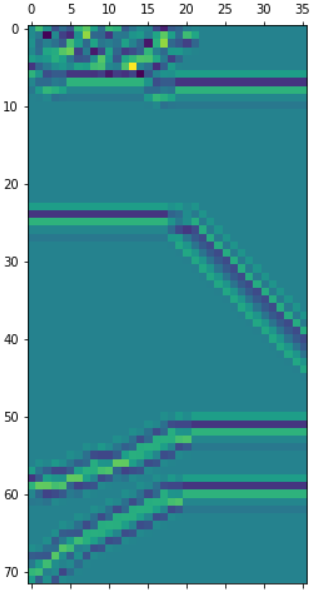
\includegraphics[width=5cm]{images/2dcnnLayer1.png}
		\caption[Bild kurz]{Add caption}
		\label{fig:vis2d1}
	\end{figure}
\end{minipage}
\begin{minipage}{0.5\textwidth}
	\begin{figure}[H]
		\centering
		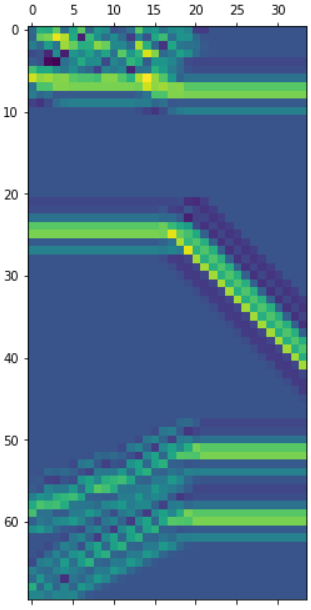
\includegraphics[width=5cm]{images/2dcnnLayer2.png}
		\caption[Bild kurz]{Add caption}
		\label{fig:vis2d2}
	\end{figure}
\end{minipage}

\begin{minipage}{0.5\textwidth}
	\begin{figure}[H]
		\centering
		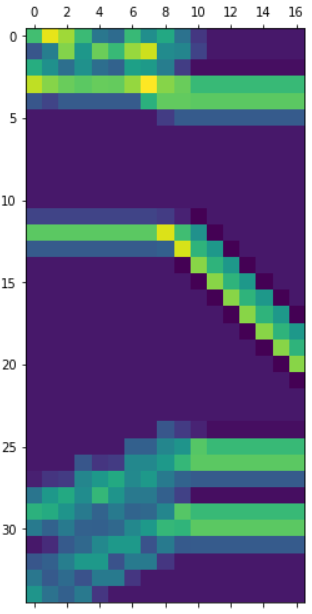
\includegraphics[width=5cm]{images/2dcnnLayer3.png}
		\caption[Bild kurz]{Add caption}
		\label{fig:vis2d3}
	\end{figure}
\end{minipage}
\begin{minipage}{0.5\textwidth}
	\begin{figure}[H]
		\centering
		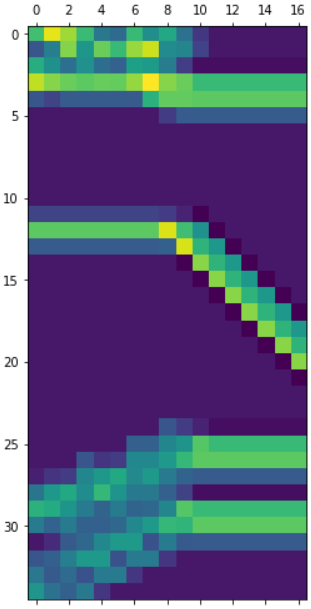
\includegraphics[width=5cm]{images/2dcnnLayer4.png}
		\caption[Bild kurz]{Add caption}
		\label{fig:vis2d4}
	\end{figure}
\end{minipage}

It can be seen that the original structure of the image is still recognizable after all convolutional, pooling and dropout layers. When dealing with cnns that have more layers, usually the original image is at some point not recognizable anymore. The remaining layers of the 2d cnn effectively opperate on one dimensionaml data and create the output. Therfore they will be left out in this vizualization.


%Especially when dealing with more copmplex structures of cnns, vizualizing all feature maps instead of one, can reveal valuable informations. Generelly, the deeper the layer, the less of the original image is recogniazable. Since the size of the 2d cnn used is comparetively small, the original image is still recognizable after all convolutional, poolind and dropout layers.  For instance can be analysed if the structure of the cnn is overly complex for the data. This is the case if the last layers do not activate anymore, as there is nothing more to learn at that point, resulting in all values of the feature maps being 0. 


%If this technique is used for actually analysisng the cnn,  



%An interesting thing about 2d cnns, what is not possible to that extend in most of the neural networks, is that the steps in between can be vizualized. As each convolutional layer creates new images using the filters, it is actually possible to look at the images between layers. Generelly the deeper the layer the less from the actual image is recognizable. It can be observed how the network step by step forms the input image to the output shape. Although this is not especially usefull for actually knowing what the network does, it is usefull for knowing if certain layers of the network do something at all. If for instance the structure of the cnn is overly complex for the data, this will be indicated by the fact that the last layers are not activating at all becuase there is nothing more to learn at that point (all values of all feature maps from a layer are 0). Although the structure of the 2d cnn used is not very complex and this technique is more relevant for larger networks, it is interesting to exemplary look at the images between the convolutions of the 2d cnn used. To do so the model is first trained for one split and then run in predict mode. When passing an image to the imput layer it is then possible to extract the images between layers.

\todo{da wird ein buch erwähnt, wo der typ erzählt wieso es gut ist das zu machen. Die zitate umschreiben in meinen text: \url{https://towardsdatascience.com/visualizing-intermediate-activation-in-convolutional-neural-networks-with-keras-260b36d60d0}}

%... bild..

%As visible, there are no layers from which all filters do not activate, meaning the structure is not overly complex for the data. 

%\todo{referenz finden und bilder einbinden von dem 2d cnn. vielleicht auch ein bild von einem größeren netz wo es nichts mehr lernt.}

\end{comment}

\section{Training and evaluation}

\begin{table}[H]
	\centering
	\caption{2D CNN. best accuracys for 5, 10, 15 and 20 steps. in brackets behind the accuiracy is the epoch.}%\label{tab1}
	\begin{tabular}{|l|l|l|l|l|}
		\hline
		Simulated Games & 5 steps & 10 steps & 15 steps& 20 steps\\
		\hline
		0 &   & && \\
		1 &  & && \\
		2 &  & && \\
		3 &  & && \\
		4 &  & && \\
		5 & &&& \\
		6 &  & && \\
		7 &  & && \\
		8 &  & && \\
		9 &  & && \\
		10 & &&& \\
		20 & &&& \\
		\hline
	\end{tabular}
\end{table}

\begin{table}[H]
	\centering
	\caption{1D CNN. best accuracys for 5, 10, 15 and 20 steps. in brackets behind the accuiracy is the epoch.}%\label{tab1}
	\begin{tabular}{|l|l|l|l|l|}
		\hline
		Simulated Games & 5 steps & 10 steps & 15 steps& 20 steps\\
		\hline
		0 &   & && \\
		1 &  & && \\
		2 &  & && \\
		3 &  & && \\
		4 &  & && \\
		5 & &&& \\
		6 &  & && \\
		7 &  & && \\
		8 &  & && \\
		9 &  & && \\
		10 & &&& \\
		20 & &&& \\
		\hline
	\end{tabular}
\end{table}

\begin{table}[H]
	\centering
	\caption{2D CNN. 20 turns. config2}%\label{tab1}
	\begin{tabular}{|l|l|l|}
		\hline
		Simulated Games & Best Accuracy (Epoch) & Best Loss (Epoch)\\
		\hline
		0 & 0.7888 (14) & 0.4822 (51) \\
		1 &  &  \\
		2 &  &  \\
		3 &  &  \\
		4 &  &  \\
		5 & 0.8450 (17) & 0.4768 (20) \\
		6 &  &  \\
		7 &  &  \\
		8 &  &  \\
		9 &  &  \\
		10 & 0.8475 (20) & 0.4796 (10) \\
		20 & 0.8437 (6) & 0.4763 (6) \\
		\hline
	\end{tabular}
\end{table}

- 1d cnn können besser mit kurzen sequencen umgehen als 2d. aber 2d sind bei mehr schritten deutlsich besser. (erste einschätzung) 

\begin{table}[H]
	\centering
	\caption{2D CNN. 20 turns. config1}%\label{tab1}
	\begin{tabular}{|l|l|l|}
		\hline
		Simulated Games & Best Accuracy (Epoch) & Best Loss (Epoch)\\
		\hline
		0 & 0.7963 (18) & 0.4931 (98) \\
		1 &  &  \\
		2 &  &  \\
		3 &  &  \\
		4 &  &  \\
		5 & 0.8437 (53) & 0.4821 (31) \\
		6 &  &  \\
		7 &  &  \\
		8 &  &  \\
		9 &  &  \\
		10 &  &  \\
		20 &  &  \\
		\hline
	\end{tabular}
\end{table}



- auch zeigen dass es sinnvoll ist simulierte daten mit zu vermwendet, also sd0x mit bestem vergleichen und so\\

- vielleiht gucken welche falsch erkannt werden und woran es liegt, also wenn die zum beispiel echt schlect oder gut sind obwohl es nicht so sein sollte (rausnhemen und gucken wie ergebnisse sind, vielleicht nur bei bestem modell)\\
- in gleichen tabellen ergebnise vor änderung am simulator und nach änderung betrachten und vergleichen\\
- training auf welchem rechner/n,was von: cpu oder gpu oder beides, hardware kurz erwähnen, vpn (fernzugriff)\\
- train test splt, leave one out k fold (+ begründung mit deep learing ..reliable results etc, randomness) \\
- kurz erklären wieso weniger züge besser sind bei dieser hci erkennung\\
- (vielleicht kram zu adaptive learning rate ändern und gucken wie es so ist, ansonsten begründen wieso ich das nicht brauche) \\
- 20 steps und 40 steps für beide trainieren mit sd0x bis sd10x plus sd20x\\
- (entweder so dass 1d cnn mit 20 steps auch konvergence erreicht oder danach nochmal anpassung von 20 steps 1d cnn damit es kovergiert)\\
- darüber schreiben dass letzen n züge nicht mehr so gut simuliert sind (zeigen) und deshalb 40 steps nicht so viel besser ist \\
- mit maximalen guten steps (glaube 16 züge oder so) trainieren und vergleichen\\
- statistical tests um signifikante unterschiede /keine unterschiede zu zeigen für verschiedene modelle etc (siehe mazens nachricht)\\
- letztlich war es wert 2D cnn auszupribieren. Werden selten für sowas verwendet haben in diesem fall aber signifank besser ergebnisse erzielt. \\
- dfalls tatsächlich btraining mit initialen daten besser ist als mit optimierten: therie könnte sein, dass durch verringerung des randomness, das netz nicht mehr so robust ist wie vorher und bei test auf den echten daten schlechter abschneidet
